% !TeX program = xelatex
\documentclass[UTF8,fontset=fandol]{ctexart}
\usepackage{amsmath, amssymb}
\usepackage{graphicx}
\usepackage{booktabs}
\usepackage[colorlinks=true, linkcolor=blue, citecolor=blue, urlcolor=blue]{hyperref}
\usepackage{bookmark}
\usepackage[margin=2.5cm]{geometry}

\title{\bfseries 蒙特卡洛流体模拟方法复现与误差评估}
\author{潘硕 PB24020526}
\date{\today}

\begin{document}

\maketitle

\begin{abstract}
蒙特卡洛（Monte Carlo, MC）方法因其在几何灵活性、点式求解和天然并行性方面的显著优势，在流体模拟及相关计算物理问题中展现出广阔的应用前景。本工作依据 Rioux-Lavoie 和 Sugimoto 等人（2022）提出的蒙特卡洛流体模拟思想，从二维无粘欧拉方程出发，逐步推广至三维 Navier--Stokes 方程，并引入方差缩减与性能优化技术，构建了三个迭代阶段的蒙特卡洛流体求解器。
Phase 1 验证了蒙特卡洛积分在二维无粘速度重建中的可行性，速度误差遵循 $O(1/\sqrt{n})$ 的统计收敛规律，而涡量演化误差主要受插值和时间离散的系统误差主导。Phase 2 将 Walk-on-Spheres（WoS）方法引入自由滑移边界流函数求解，实现了无网格边界处理，守恒性优于传统差分法，但计算成本显著增加，高阶时间格式未能进一步改善精度。Phase 3 将算法扩展至三维黏性流动，成功复现了 Taylor--Green 涡旋中拟涡能先升后降的演变趋势，但定量偏差较大。
综合而言，蒙特卡洛方法在无网格计算和复杂边界处理方面具有独特优势，但其精度和计算效率尚不及传统确定性方法；未来通过方差缩减、混合算法及硬件加速等手段，有望在湍流等复杂问题中成为有效补充。
\end{abstract}

\section{引言及相关工作}

\subsection{引言}
蒙特卡洛方法在光线传输和几何处理中已展示了其处理复杂几何和高维积分的能力。Rioux-Lavoie等（2022）将其引入流体模拟，
通过涡量输运方程避免了压力投影的全局求解。本项目分三个阶段逐步实现并评估该方法：Phase 1（2D无粘欧拉）、Phase 2（2D自由滑移边界）、Phase 3（3D Navier-Stokes）。本报告将给出各阶段的算法描述、实验对比和误差分析。
\section{相关工作}

本文融合了蒙特卡洛积分、无网格PDE求解、涡量流体模拟及Navier–Stokes方程的概率表示等多个方向。

\begin{enumerate}
    \item 蒙特卡洛方法在渲染中已取得巨大成功（Kajiya，1986；Cook，1986；Pharr等，2018），其无网格特性启发了几何处理领域采用Walk-on-Spheres（WoS）求解边界值PDE（Sawhney和Crane，2020；Sawhney等，2022）。我们借鉴此思路，将WoS应用于流体模拟中的流函数泊松方程，但直接基于Muller（1956）的原始方法，而非其变体。
    \item 流体模拟方面，欧拉方法（Stam，1999；Fedkiw等，2001）、拉格朗日方法（Desbrun和Gascuel，1996；Müller等，2003）及混合方法（Zhu和Bridson，2005；Jiang等，2015）均依赖空间离散。涡量形式可导出涡粒子方法（Chorin，1973；Cottet和Koumoutsakos，2000），图形学中有多种改进（Park和Kim，2005；Brochu等，2012）。我们同样采用涡量和Biot–Savart律，但将其转化为适于MC估计的递归积分形式。
    \item 在概率模型方面，Busnello等（2005）和Constantin与Iyer（2007）给出了Navier–Stokes方程的随机表示，但此前未见实际数值模拟。我们基于Feynman–Kac公式构建了处理黏性和涡拉伸的随机时间推进方案，与格子Boltzmann方法（Li等，2018）的本质区别在于我们无需空间格点。
\end{enumerate}

\section{整体框架与阶段划分}
项目分为三个独立子项目（Phase 1--3），每个阶段在上一阶段基础上增加物理复杂性或数值技术，如表\ref{tab:phases}所示。

\begin{table}[htbp]
\centering
\caption{各阶段特性对比}
\label{tab:phases}
\begin{tabular}{lccccc}
\toprule
Phase & 方程 & 维度 & 边界 & 粘性 & 拉伸 \\
\midrule
1 & 欧拉 & 2D & 无 & -- & -- \\
2 & 欧拉 & 2D & 自由滑移 & -- & --\\
3 & NS & 3D & 无（开放域） & $\checkmark$ & $\checkmark$ \\ 
\bottomrule
\end{tabular}
\end{table}

核心思想：使用涡量作为原始变量，通过Biot-Savart定律重建速度场，利用网格缓存存储历史涡量避免递归爆炸，并通过半拉格朗日后向追踪推进时间演化。

\section{Phase 1：二维无粘蒙特卡洛流体模拟}

Phase 1 实现了二维不可压缩无粘欧拉方程的蒙特卡洛求解器，其核心在于利用涡量-速度形式的欧拉方程，将流体的时间推进与速度重建解耦。
\subsection{算法原理}
\begin{enumerate}
    \item \textbf{涡量输运方程}：对于无粘不可压缩流动，流体的涡量沿流线守恒，即物质导数 $D\omega/Dt = 0$。为获得查询点（例如输出图像像素或网格节点）在时刻 $t$ 的涡量，本文采用后向轨迹追踪法，即从当前点 $\mathbf{x}$ 沿时间反向追踪至前一时刻 $t-\Delta t$，其位置近似为：
    \[
    \boldsymbol{\omega}(t, \mathbf{x}) \approx \boldsymbol{\omega}\bigl(t - \Delta t,\; \mathbf{x} - \mathbf{v}(t - \Delta t, \mathbf{x})\,\Delta t\bigr)
    \]
    其中速度场 $\mathbf{v}$ 来自上一时刻的重建结果。

    \item \textbf{速度重建}：给定涡量场 $\omega(\mathbf{y})$，速度 $\mathbf{v}(\mathbf{x})$ 可通过 Biot–Savart 积分求得。在二维情形下，涡量为标量（垂直于平面），速度场满足 $\omega = \nabla \times \mathbf{v}$，其显式形式为：
    \[
    \mathbf{v}(\mathbf{x}) = \int_{\Omega} \omega(\mathbf{y})\, \mathbf{G}(\mathbf{x} - \mathbf{y})\, \mathrm{d}\mathbf{y},
    \qquad 
    \mathbf{G}(\mathbf{r}) = \frac{1}{2\pi}\frac{(-\mathbf{r}_y,\; \mathbf{r}_x)}{|\mathbf{r}|^2},
    \]
    其中 $\mathbf{r} = \mathbf{x} - \mathbf{y}$。该核函数具有奇异性，但在数值积分中可通过解析处理或正则化避免。

    \item \textbf{蒙特卡洛估计}：由于 Biot–Savart 积分在全域 $\Omega$ 上定义，解析计算困难，因此采用蒙特卡洛方法进行数值估计。引入重要性采样分布 $p(\mathbf{y}\,|\,t,\mathbf{x})$，从该分布中抽取 $n_{\mathrm{mc}}$ 个独立样本 $\{\mathbf{y}_i\}_{i=1}^{n_{\mathrm{mc}}}$，则速度的无偏估计为：
    \[
    \langle \mathbf{v}(t, \mathbf{x}) \rangle = \frac{1}{n_{\mathrm{mc}}} \sum_{i=1}^{n_{\mathrm{mc}}} 
    \frac{\omega(t, \mathbf{y}_i)\, \mathbf{G}(\mathbf{x} - \mathbf{y}_i)}{p(\mathbf{y}_i\,|\,t,\mathbf{x})}.
    \]
    为了降低方差，通常选择与核函数形状相近的分布，例如基于距离的密度或均匀分布。
\end{enumerate}

\subsection{算法实现}

依据上述原理，编写了基于网格化涡量场的 Biot–Savart 速度重建程序。该程序接收离散网格上的涡量值，对任意查询点（或查询点集合）计算速度估计值。
为了提高计算效率，利用 Numba 即时编译技术对循环进行并行加速，同时采用向量化操作处理多个查询点。

\subsection{误差分析（Taylor–Green 涡旋）}

\subsubsection{模拟设置}

Taylor–Green 涡旋是二维不可压 Navier–Stokes 方程的一个经典解析特解，其无粘情形下涡量保持初始分布平流，具有精确的解析解，常用于验证数值方法的准确性。初始涡量场取为：
\[
\omega(x,y) = 2\cos(\pi x)\cos(\pi y),
\]
定义在周期性方域 $[0,2]\times[0,2]$ 上。模拟参数如表~\ref{tab:参数} 所示。

\begin{table}[htbp]
\centering
\caption{模拟参数设置}
\label{tab:参数}
\begin{tabular}{lccc}
\toprule
采样分辨率 & 时间步长 ($s$) & 总模拟时间 ($s$) & 粘度系数 \\
\midrule
32 $\times$ 32 & 0.05 & 1 & 0.0（无粘）\\
\bottomrule
\end{tabular}
\end{table}

\subsubsection{模拟结果}

我们统计了初始时刻速度场的 $L_2$ 误差以及末态（$t=1$s）涡量场的 $L_2$ 误差，结果如表~\ref{tab:nmc1} 所示。

\begin{table}[htbp]
\centering
\caption{不同样本数下的误差}
\label{tab:nmc1}
\begin{tabular}{lccc}
\toprule
$n_{\mathrm{mc}}$ & 初始速度 $L_2$ 误差 & 涡量演化 $L_2$ 误差 \\
\midrule
128  & 0.832577 & 0.110724 \\
256  & 0.556695 & 0.098925 \\
512  & 0.397681 & 0.086644 \\
1024 & 0.371951 & 0.081752 \\
2048 & 0.219085 & 0.080729 \\
4096 & 0.166523 & 0.075593 \\
\bottomrule
\end{tabular}
\end{table}

\begin{figure}[htbp]
\centering
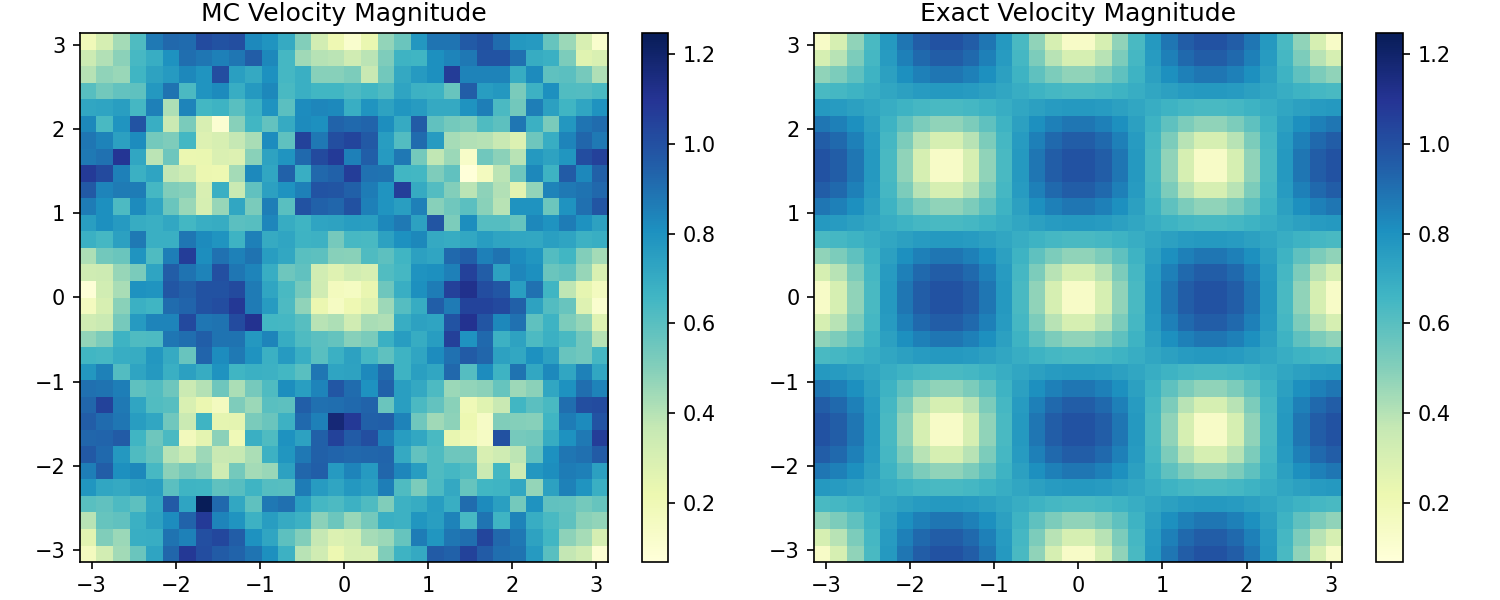
\includegraphics[width=0.9\textwidth]{../pic/step1/tg2d_velocity_magnitude.png}
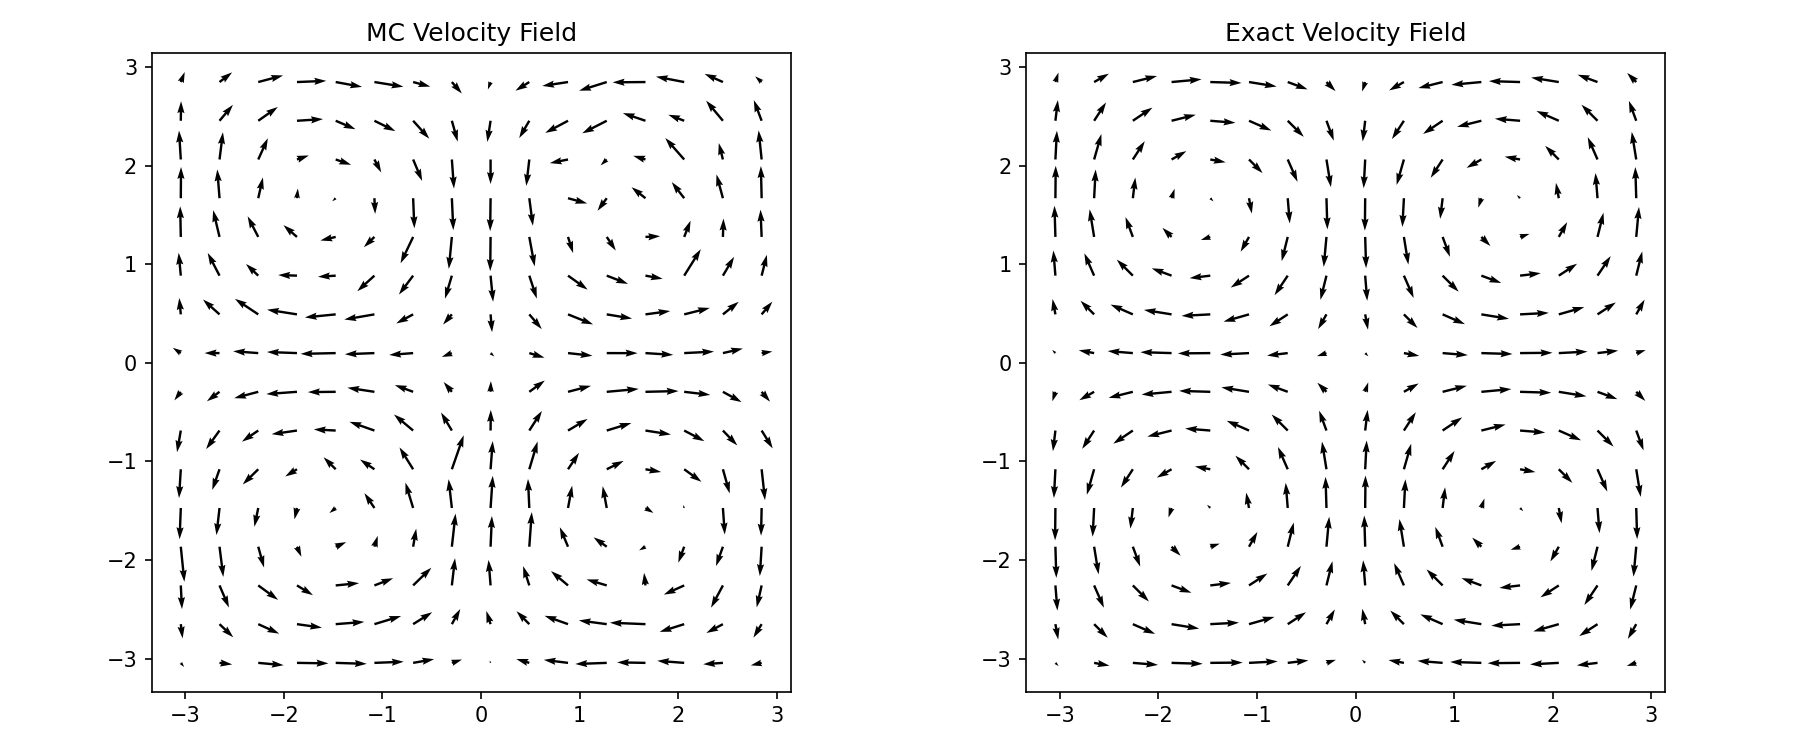
\includegraphics[width=0.9\textwidth]{../pic/step1/tg2d_velocity_quiver.png}
\caption{速度场重建结果（$n_{\mathrm{mc}}=2048$，$64\times64$ 网格）}
\label{fig:phase1_velocity}
\end{figure}

由表可见：
\begin{enumerate}
    \item 速度 $L_2$ 误差随样本数 $n_{\mathrm{mc}}$ 增加而单调下降（从 0.83 降至 0.17），其下降速率与 $O(1/\sqrt{n_{\mathrm{mc}}})$ 的蒙特卡洛统计误差规律相符。这表明速度误差主要由 MC 噪声主导，可通过增加样本量有效降低。
    \item 涡量演化 $L_2$ 误差随样本数增加仅缓慢下降（从 0.11 降至 0.076），说明该误差主要来源于系统误差（如时间离散和空间插值耗散），而非统计噪声。
\end{enumerate}

\subsection{改进措施}

为进一步提高模拟精度，本文从时间步长和网格分辨率两方面进行探究。

\subsubsection{改变时间步长}

固定样本数 $n_{\mathrm{mc}}=2048$ 及其他参数，仅改变时间步长 $dt$，计算末态涡量场的 $L_2$ 误差，结果如表~\ref{tab:time} 所示。

\begin{table}[htbp]
\centering
\caption{时间步长对涡量演化误差的影响（$n_{\mathrm{mc}}=2048$）}
\label{tab:time}
\begin{tabular}{lcc}
\toprule
$dt$ (s) & 涡量演化 $L_2$ 误差 \\
\midrule
0.1   & 0.060387 \\
0.05  & 0.047257 \\
0.02  & 0.051737 \\
0.01  & 0.076589 \\
0.005 & 0.120662 \\
\bottomrule
\end{tabular}
\end{table}

当 $dt$ 较大（如 0.1 s）时，总步数很少（$T/dt = 10$ 步），MC 噪声累积时间短，此时误差主要由时间离散误差主导，因此 $dt$ 从 0.1 减小至 0.05 时误差下降。
然而，当 $dt$ 继续减小（0.02、0.01、0.005）时，总步数剧增（分别 50、100、200 步），每一步的插值误差和 MC 噪声不断累积，
最终压过了时间离散精度的提升，导致总误差反而增大。综合考虑，选取 $dt = 0.05$ s 作为默认时间步长。

\subsubsection{增大网格分辨率}

固定 $dt = 0.05$ s，总时间 $t = 0.5$ s，样本数 $n_{\mathrm{mc}}=2048$，改变空间网格分辨率，统计末态涡量误差，如表~\ref{tab:grid} 所示。

\begin{table}[htbp]
\centering
\caption{网格分辨率对误差的影响（$n_{\mathrm{mc}}=2048$）}
\label{tab:grid}
\begin{tabular}{lcc}
\toprule
$nx \times ny$ &  涡量演化 $L_2$ 误差 \\
\midrule
32 $\times$ 32  &  0.284370 \\
64 $\times$ 64  &  0.118122 \\
128 $\times$ 128 & 0.044410 \\
256 $\times$ 256 & 0.019178 \\
512 $\times$ 512 &  0.014771 \\
\bottomrule
\end{tabular}
\end{table}



结果表明，提高网格分辨率能够显著降低涡量演化误差（从 0.284 降至 0.015），这验证了空间精度对涡量输运的重要性。

\subsection{算法总结}

Phase 1 构建了一个基于蒙特卡洛积分的二维无粘欧拉方程求解器，其核心创新在于使用随机采样替代传统网格上的确定性积分，从而避免了全局卷积的显式计算。该算法具有以下特点：
\begin{itemize}
    \item \textbf{无网格灵活性}：速度重建可在任意查询点独立进行，便于与粒子追踪或非结构化输出相结合。
    \item \textbf{易于并行}：每个查询点的速度估计相互独立，非常适合 GPU 或大规模并行架构。
    \item \textbf{统计误差可预测}：速度误差随样本数平方根衰减，可通过增加样本数精确控制。
\end{itemize}
然而，当前实现也暴露了明显不足：
\begin{itemize}
    \item \textbf{系统误差累积}：涡量输运阶段的时间离散和空间插值引入的耗散会随时间步增加而放大，限制了长时间模拟的精度。
    \item \textbf{计算成本}：为达到较高精度，需要大量样本（如 $n_{\mathrm{mc}}>4000$），导致单步计算开销较大。
\end{itemize}

\section{Phase 2：带自由滑移边界的蒙特卡洛流体模拟}
Phase 2 实现在自由滑移边界下的二维不可压缩无粘欧拉方程的蒙特卡洛求解器。
\subsection{算法原理}

\begin{enumerate}
    \item \textbf{流函数法}：引入流函数 $\Psi$，使得速度场 $\mathbf{v}$ 可以表示为流函数 $\Psi$ 的旋度：
\[\mathbf{v} = -\nabla \times \Psi\]
在二维自由滑移边界下，边界速度的法向方向分量为0，取 Dirichlet 边界条件 $\Psi|_{\text{边界}}=0$。

代入涡量表达式 $\boldsymbol{\omega} = \nabla \times \mathbf{v}$，有：
\[\nabla^2 \Psi = -\boldsymbol{\omega}\]

    \item \textbf{Walk-on-Sphere (WoS) 方法}：WoS算法是一种无网格的蒙特卡洛数值方法，通过在求解域内构造的最大球面上反复随机跳跃来模拟布朗运动，并将偏微分方程（如拉普拉斯方程）的解近似表示为随机游走首次命中边界值的统计期望。
    
    使用 WoS 方法求解满足 Dirichlet 边界条件的泊松方程：
    \[\nabla^2 \Psi = -\boldsymbol{\omega}\]
    \[\Psi|_{\text{边界}} = 0\]
\end{enumerate}

\subsection{算法实现}
将 Phase 1 中的半拉格朗日涡量平流和 Biot–Savart 速度重建模块与 WoS 流函数求解器耦合，构建了完整的 Phase 2 求解器。每个时间步的流程如下：
\begin{enumerate}
    \item 根据当前涡量场，利用 WoS 方法求解泊松方程 $\nabla^2 \Psi = -\omega$，获得流函数分布；(参考\url{https://github.com/nv-tlabs/wosx})
    \item 由流函数差分或解析梯度计算速度场 $\mathbf{v}$；
    \item 使用半拉格朗日后向追踪更新涡量场至下一时刻；
    \item 重复直至模拟结束。
\end{enumerate}

所有关键循环均使用 Numba 加速。

\subsection{性能评估}
\subsubsection{模拟设置}
选取一个包含中央圆柱形障碍物的方形区域$([-1 , 1]^2)$，障碍物半径为0.1，初始条件设为关于原点对称的两个圆形涡旋，涡旋强度满足高斯分布，中心位于$(\pm 0.5, 0)$处，
如图\ref{fig:init}所示。

作为对比，我们同时使用经典的有限差分流函数法（直接求解 $\nabla^2\Psi=-\omega$ 的线性方程组，记为 Grid）和本 Monte Carlo 方法（记为 WoSX）进行相同条件(表\ref{tab:参数2})下的模拟。

\begin{table}[htbp]
\centering
\caption{模拟参数设置}
\label{tab:参数2}
\begin{tabular}{lcccc}
\toprule
采样分辨率 & 时间步长 ($s$) & 总模拟时间 ($s$) & 中心障碍物半径 & nmc\\
\midrule
64 $\times$ 64& 0.05 & 3 & 0.1 & 2048\\
\bottomrule
\end{tabular}
\end{table}

\begin{figure}
\centering
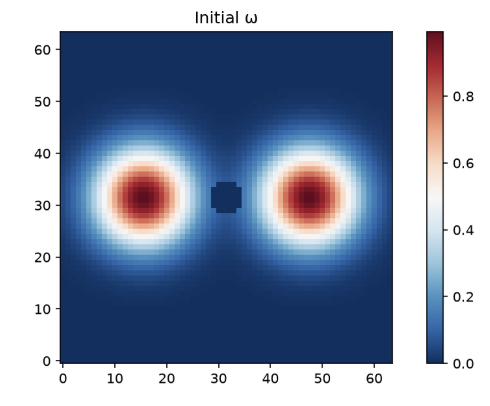
\includegraphics[width=0.4\textwidth]{../pic/step2/init.png}
\caption{流场初始条件示意图}
\label{fig:init}
\end{figure}

\subsubsection{模拟结果}

\begin{figure}
\centering
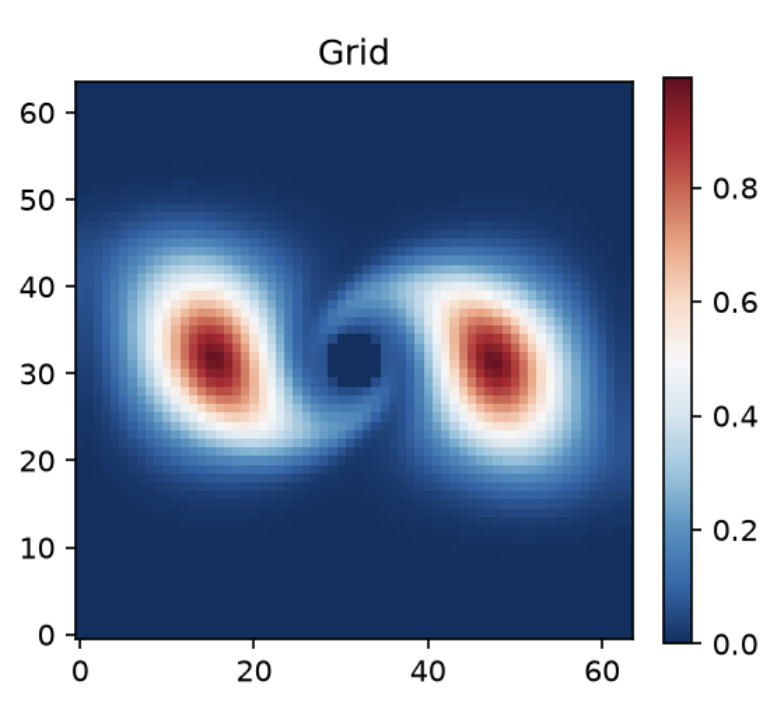
\includegraphics[width=0.4\textwidth]{../pic/step2/grid.png}
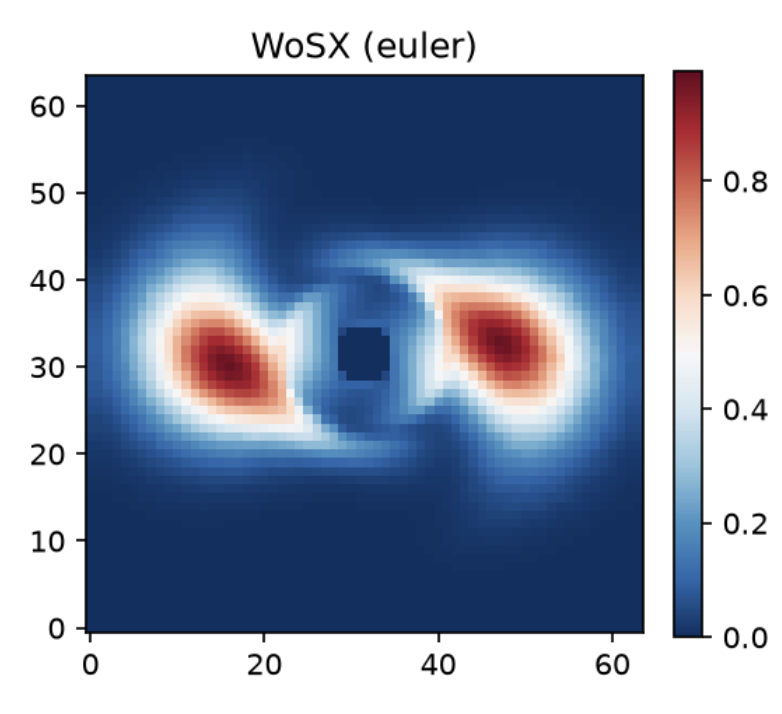
\includegraphics[width=0.4\textwidth]{../pic/step2/wosx.png}
\caption{MC方法与网格流函数法在自由滑移边界下的涡量分布对比（64$\times$64网格，$dt=0.05$，$T=3$s）}
\label{fig:grid_wosx}
\end{figure}

\begin{figure}
\centering
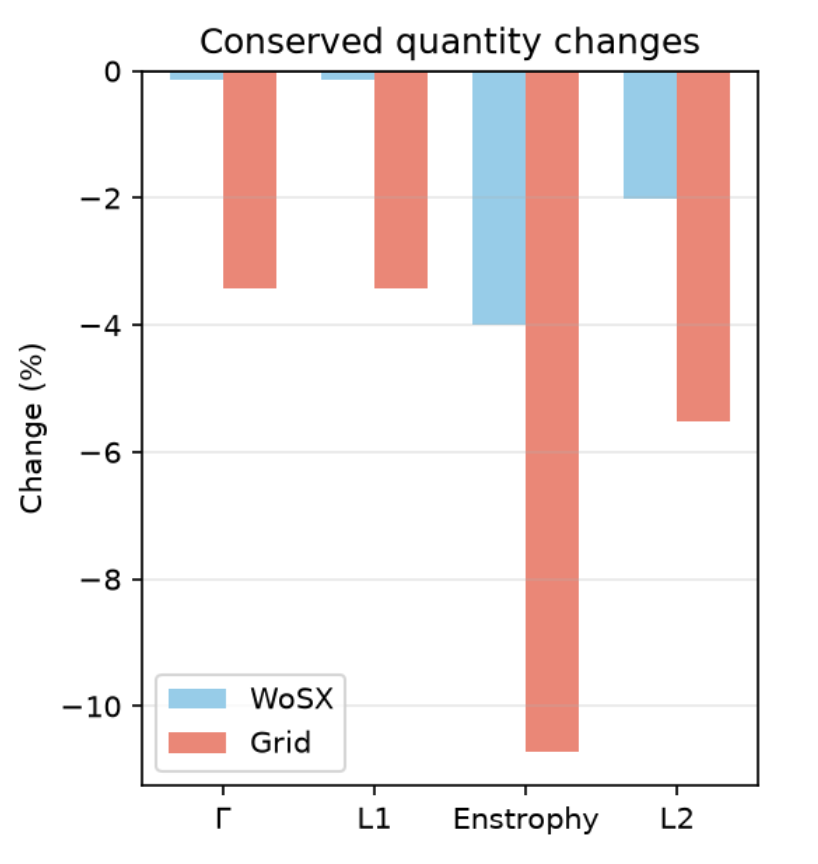
\includegraphics[width=0.4\textwidth]{../pic/step2/changes.png}
\caption{MC方法与网格流函数法在自由滑移边界下的守恒量变化（64$\times$64网格，$dt=0.05$，$T=3$s）}
\label{fig:changes}
\end{figure}

模拟结果如图\ref{fig:grid_wosx}所示。计算两种方法末态的流体总环量及拟涡量守恒量，统计结果如图\ref{fig:changes}所示。

图~\ref{fig:grid_wosx} 展示了两种方法在 $t=3$s 时的涡量分布。可以看出，Grid 方法得到的涡量场略为平滑（耗散稍大），而 WoSX 方法保留更多细碎结构，但伴随一定的随机噪声。

WoSX 在时间推进中数值耗散略小、守恒性稍好，但计算代价高；Grid 流函数法快速但涡量衰减略大。两者差异可能源于随机游走噪声或边界处理方式的不同。

\subsection{改进措施}
为降低半拉格朗日平流中的数值耗散，我们尝试引入两种改进方案：二阶 Runge–Kutta 后向追踪（RK2）和 MacCormack 误差校正方法。

\subsubsection{MacCormack方法}
MacCormack 方法的具体步骤为：
\begin{enumerate}
    \item 用标准半拉格朗日法（一阶 Euler 后向追踪）将涡量场平流一步，得到预测场 $\omega^A$；
    \item 使用同一速度场，将 $\omega^A$ 反向平流回原位，得到 $\omega^B$；
    \item 利用预测与反向结果的差异修正原结果：
    \[
    \omega^{\text{new}} = \omega^A + \frac{1}{2}\left(\omega - \omega^B\right).
    \]
\end{enumerate}

该方法可在几乎不增加额外信息的前提下抵消一阶格式的部分截断误差，从而改善守恒性。
\subsubsection{模拟结果}

我们固定 WoS 求解器（$n_{\mathrm{mc}}=2048$），分别使用四种平流方案：
\begin{itemize}
    \item Grid：直接用有限差分求解流函数（非 WoS），平流采用一阶 Euler 后向追踪；
    \item Euler：WoS + 一阶 Euler 后向追踪；
    \item RK2：WoS + 二阶 Runge–Kutta 后向追踪；
    \item Mac：WoS + MacCormack 校正。
\end{itemize}

统计末态总环量和拟涡量的相对变化以及运行时间，结果如表~\ref{tab:scheme} 所示。

\begin{table}
\centering
\caption{不同算法下的运行参数}
\label{tab:scheme}
\begin{tabular}{lcccc}
\toprule
方法 & 时间步长 & 总环量 & 拟涡量 & 运行时间($s$)\\
\midrule
grid & 0.05 & -3.42\% & -10.72\% & 5.85\\
euler & 0.05 & -0.14\% & -3.99\% & 234.94\\
RK2 &  0.05 & -0.22\% & -4.05\% & 246.38\\
Mac &  0.05 & -0.29\% & -3.93\% & 400.83\\
\bottomrule
\end{tabular}
\end{table}

结果显示：
\begin{itemize}
    \item 相较于传统 Grid 方法，所有 WoS 类方法均显著提升了守恒性，这表明 WoS 流函数求解器在边界处理上引入的数值耗散更小。
    \item 在 WoS 框架内，RK2 和 MacCormack 方法相比一阶 Euler 并未带来明显改善。这可能是因为 WoS 自身的随机噪声已经掩盖了高阶时间格式带来的精度增益，或者边界附近的距离计算误差主导了整体误差。
    \item 计算成本方面，MacCormack 因需两次平流操作，耗时约为 Euler 的两倍，而 RK2 运行结果与 euler 相近。
\end{itemize}

因此，在实际应用中，一阶 Euler 后向追踪结合 WoS 已能获得良好的折衷效果，而高阶格式在当前框架下并不划算。
\subsection{结果分析}
Phase 2 成功将 WoS 方法应用于带自由滑移边界的二维无粘流动模拟，实现了复杂几何下的无网格流函数求解。与网格流函数法相比，WoS 方法在保持守恒性方面具有优势，这源于其无需对边界附近网格进行特殊处理，避免了传统有限差分中的局部截断误差。然而，WoS 的计算代价高昂（约为 Grid 方法的 40 倍），且其随机性导致流场中存在可见噪声，影响涡量场的平滑性。

高阶时间格式（RK2、MacCormack）未能进一步提升精度，说明当前瓶颈可能在于空间离散（插值）和 WoS 估计的方差，而非时间离散。
未来工作可考虑：
\begin{enumerate}
    \item 引入方差缩减技术（如控制变量）降低 WoS 的统计噪声；
    \item 探索自适应 WoS 样本分配，在边界附近增加采样密度以提升局部精度
\end{enumerate}

总体而言，Phase 2 验证了 WoS 在含障碍物流动中的可行性，为后续处理更复杂边界条件（如无滑移或周期边界）及三维拓展奠定了基础。

\section{Phase 3：三维Navier-Stokes蒙特卡洛模拟}

本节将蒙特卡洛方法推广至三维不可压缩黏性流动，构建了三维 Navier–Stokes 方程的蒙特卡洛求解器。
与二维无粘情形相比，三维流动中涡量不仅平流输运，还受到涡拉伸和黏性扩散的共同作用，物理过程更加丰富，数值模拟也更具挑战性。

\subsection{算法原理}
三维情形下的涡量传输方程可以表示为：
\[ \frac{D \mathbf{\omega}}{D t} = (\mathbf{\omega} \cdot \nabla) \mathbf{v} + \nu \nabla^2 \mathbf{\omega} \]

利用Feynman-Kac公式处理，涡量运输方程的解满足：

\[\mathbf{\omega(\bar{t}, \bar{x})} = \mathbb{E} [U_{\bar{t}} \mathbf{\omega}(0, X_{\bar{t}})|U_0 = I, X_0 = \bar{x}]\]

这个期望的意义是，在初始时刻 $t=0$，所有可能的随机轨迹 $X_s$ 及其对应的变形矩阵 $U_t$ 的期望，恰好等于 $\bar{t}$ 时刻 $\bar{\mathbf{x}}$ 处的涡量。

对上述公式进行时间离散化，时间步长设为 $\Delta s = t / n$，得到三个子步骤：

\begin{enumerate}
    \item \textbf{平流}：半拉格朗日后向追踪；
    \[\mathbf{x}_a = \mathbf{x} - \Delta t \mathbf{v}(t - \Delta t, \mathbf{x})\]

    \item \textbf{扩散}：叠加高斯扰动 $\sqrt{2\nu\Delta t}\xi$；
    \[\mathbf{x}_b \sim \mathcal{N} (\mathbf{x}_a , \sqrt{2\nu\Delta t} I), i = 1, \cdots, n_d\]

    \item \textbf{拉伸}：通过速度差分离散应变率张量作用。
    \[U_{j+1} = \left[ I + \Delta t \, D_{\mathbf{v}}(t_j, X_{\bar{t} - t_j}) \right] U_j, \quad U_0 = I\]

    用离散的涡量近似计算 $D_{\mathbf{v}} \boldsymbol{\omega}$：
    \[D_{\mathbf{v}} \boldsymbol{\omega}(t, \mathbf{x}) \approx \frac{|\boldsymbol{\omega}(t, \mathbf{x})|}{h} \left[ \mathbf{v}(t, \mathbf{x} + \overrightarrow{\Delta x}) - \mathbf{v}(t, \mathbf{x} - \overrightarrow{\Delta x}) \right]\]
\end{enumerate}

给定初始条件 $\mathbf{\omega}(0, \cdot)$，利用 Monte Carlo 采样计算 $\boldsymbol{\omega}(t_i, \mathbf{x}_i)$ 的值：

\[\boldsymbol{\omega}(t_i, \mathbf{x}_i) \approx \frac{1}{n_d} \sum_{j=1}^{n_d} \left[ \boldsymbol{\omega}(t_{i-1}, \mathbf{x}_{i-1}^j) + \Delta t \, \langle D_{\mathbf{v}} \boldsymbol{\omega}(t_{i-1}, \mathbf{x}_{i-1}^j) \rangle \right]\]

\subsection{算法实现}

基于前述离散格式，我们构建了三维蒙特卡洛 Navier–Stokes 求解器，分别完成了平流、扩散及拉伸子模块的实现，并借助 Numba 的并行计算能力对核心循环进行了加速优化。

\subsection{误差评估：3D Taylor-Green涡旋}

\subsubsection{模拟设置}

三维 Taylor–Green 涡旋是验证黏性流动数值方法的经典基准问题。其初始速度场为
\[
\begin{cases}
u = \sin(x)\cos(y)\cos(z), \\[4pt]
v = -\cos(x)\sin(y)\cos(z), \\[4pt]
w = 0,
\end{cases}
\]

定义在周期方盒 $[-\pi,\pi]^3$ 上。该初始场会因涡拉伸产生小尺度结构，随后黏性耗散导致动能衰减，拟涡能（enstrophy）先升后降，是检验算法捕捉转捩和耗散能力的关键测试。

模拟参数如表\ref{tab:参数3}所示。

\begin{table}[htbp]
\centering
\caption{模拟参数设置}
\label{tab:参数3}
\begin{tabular}{lcccc}
\toprule
采样分辨率 & 时间步长 ($s$) & 总模拟时间 ($s$) & 粘度 &nmc \\
\midrule
64 $\times$ 64& 0.1 & 20 & 0.000625 & 1024\\
\bottomrule
\end{tabular}
\end{table}

\subsubsection{算法评估}
作为对比基准，我们采用公开的benchmark 数据文件作参考（参考解）。主要统计量为总动能 $E_k = \frac{1}{2}\int |\mathbf{v}|^2 \,\mathrm{d}V$ 和拟涡能 $\mathcal{Z} = \frac{1}{2}\int |\boldsymbol{\omega}|^2 \,\mathrm{d}V$，
结果如图\ref{fig:step3_enstroph}所示。

\begin{figure}
\centering
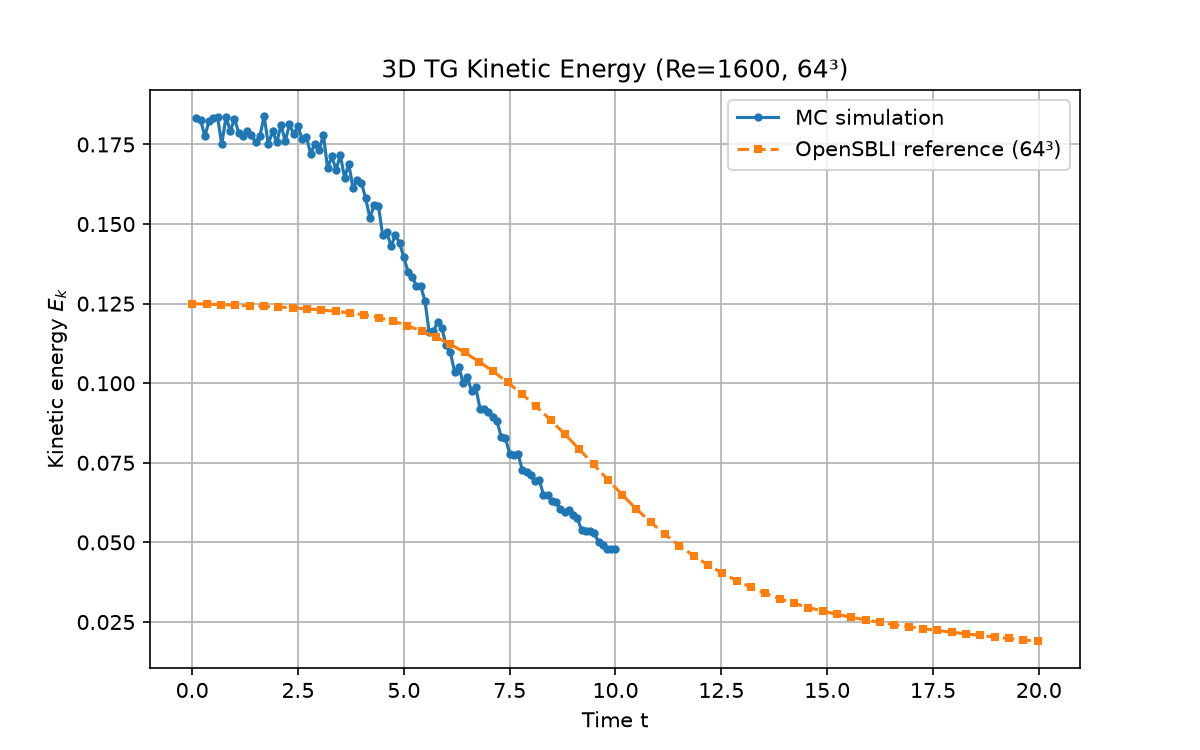
\includegraphics[width=0.5\textwidth]{../pic/step3/tg3d_Ek_comparison.png}
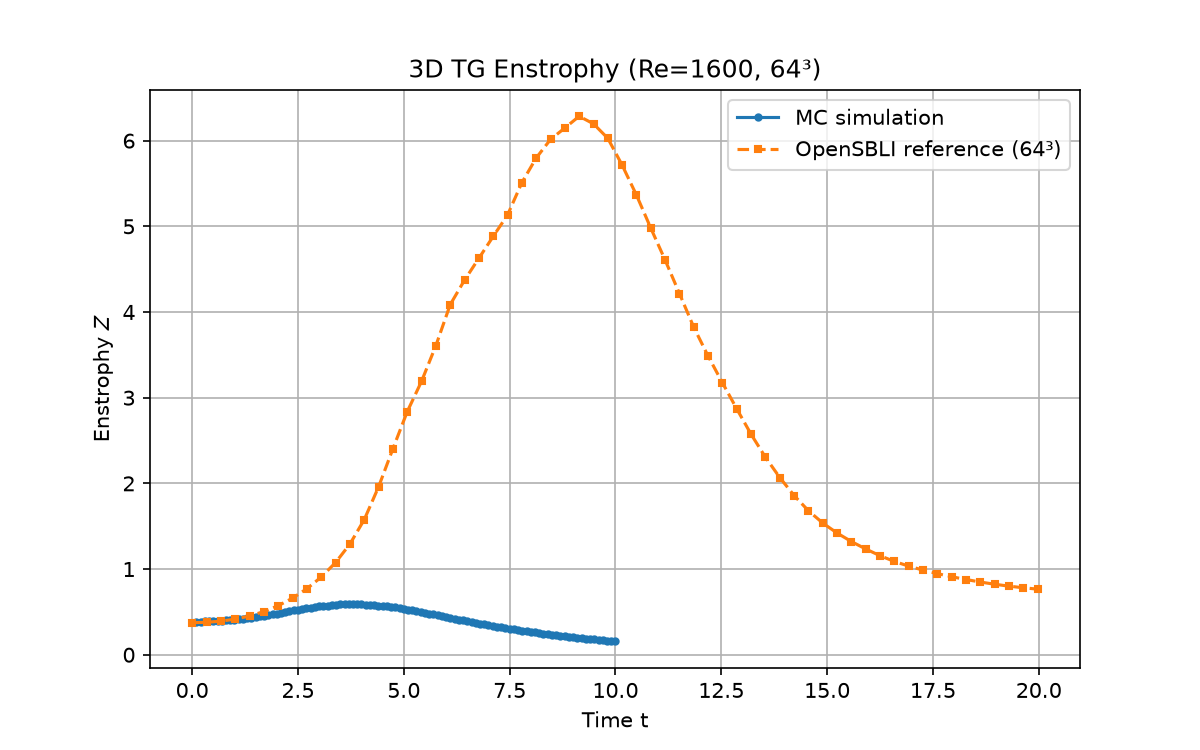
\includegraphics[width=0.5\textwidth]{../pic/step3/tg3d_Z_comparison.png}
\caption{Phase 3 3D Taylor-Green 拟涡能随时间变化曲线 （64$^3$网格，$dt=0.1$，$T=10$s，$\nu=0.000625$）}
\label{fig:step3_enstroph}
\end{figure}

从图中可以看出：
\begin{itemize}
    \item 本算法能够定性再现 Taylor–Green 涡旋的主要演化特征——拟涡能在初期迅速上升（涡拉伸占优），随后因黏性耗散而缓慢下降。
    \item 然而，定量上存在明显偏差：本算法得到的拟涡能峰值提前出现（约 $t=4$ s vs. 基准的 $t=8$ s），且峰值偏低；动能衰减速率也快于基准。
\end{itemize}

这种偏差主要源于以下数值误差的累积效应：
\begin{enumerate}
    \item \textbf{插值耗散}：半拉格朗日追踪中的三线性插值引入了数值黏性，人为加速了能量从解析尺度向亚网格尺度的传递。
    \item \textbf{拉伸项离散误差}：有限差分估计速度梯度时，$h$ 的选取对拉伸大小敏感，过大会低估拉伸，过小则放大噪声，难以兼顾。
    \item \textbf{蒙特卡洛噪声}：有限样本数导致拉伸和扩散估计存在统计涨落，该噪声与时间推进耦合，可能引起不稳定或过早耗散。
\end{enumerate}

\subsection{算法总结}

Phase 3 将蒙特卡洛方法扩展至三维黏性 Navier–Stokes 方程，构建了包含平流、扩散和拉伸三算子分裂的随机求解器。

尽管其定量精度有待提高，但本算法成功捕获了三维涡量输运的核心物理机制，证明了蒙特卡洛框架在三维黏性流动中的可行性。

\section{总结}

本框架展现了蒙特卡洛方法在无网格计算、复杂几何边界处理以及三维黏性流动模拟中的潜力，但其精度和计算效率目前尚不及传统确定性方法。未来通过方差缩减、混合算法和硬件加速等手段，有望在湍流等复杂问题中成为传统方法的有效补充。

\section{未来与展望}

基于当前工作的分析与不足，我们规划从以下方向进一步推进：

\begin{itemize}
    \item \textbf{算法框架拓展}：引入速度算子分裂策略，结合 Walk-on-Boundary 方法进行投影步求解，从而在保持无网格优势的同时，更自然地处理无滑移边界条件，提升方法的工程适用性。
    \item \textbf{方差缩减策略}：引入控制变量、分层采样和准蒙特卡洛等高级方差缩减技术，有效降低蒙特卡洛估计的统计噪声，加速收敛速度，减少达到给定精度所需的样本量。
    \item \textbf{三维 Biot–Savart 积分加速}：结合快速多极子方法（FMM）或树状算法，将三维速度重建的复杂度从 \(O(N^2)\) 降至 \(O(N \log N)\)，从而支撑更高分辨率和更多样本的大规模模拟。
    \item \textbf{高性能并行实现}：充分利用 GPU 的众核架构和蒙特卡洛方法的天然并行性，将每个随机轨迹和查询点独立映射至线程，实现极致的并行扩展，为实时或交互式应用奠定基础。
\end{itemize}

上述方向旨在系统性地解决当前框架在精度、效率和边界处理方面的核心瓶颈，推动蒙特卡洛方法在复杂流体模拟中的实际应用。

\section{致谢}

衷心感谢方清老师在项目研究过程中给予的宝贵意见和悉心指导，其专业见解为本文工作的顺利开展提供了重要支撑。同时，诚挚感谢侍子译同学在蒙特卡洛方法应用于流体模拟方面所提供的深入讨论与有益建议，其热情帮助与学术交流对本文的完善起到了积极作用。

\begin{thebibliography}{15}

\bibitem{brochu2012} Brochu T, Keeler T, Bridson R. Linear-time smoke animation with vortex sheet meshes[C]//Proceedings of the ACM SIGGRAPH/Eurographics Symposium on Computer Animation. 2012.

\bibitem{busnello2005} Busnello B, Flandoli F, Romito M. A probabilistic representation for the vorticity of a three-dimensional viscous fluid[J]. Proceedings of the Edinburgh Mathematical Society, 2005, 48(2): 295--336.

\bibitem{chorin1973} Chorin A J. Numerical study of slightly viscous flow[J]. Journal of Fluid Mechanics, 1973, 57(4): 785--796.

\bibitem{constantin2007} Constantin P, Iyer G. A stochastic Lagrangian representation of the 3D Navier-Stokes equations[J]. Communications on Pure and Applied Mathematics, 2007, 61(3): 330--345.

\bibitem{cook1986} Cook R L. Stochastic sampling in computer graphics[J]. ACM Transactions on Graphics, 1986, 5(1): 51--72.

\bibitem{cottet2000} Cottet G-H, Koumoutsakos P D. Vortex methods: theory and practice[M]. Cambridge University Press, 2000.

\bibitem{desbrun1996} Desbrun M, Gascuel M-P. Smoothed particles: A new paradigm for animating highly deformable bodies[C]//Computer Animation and Simulation'96. Springer, 1996: 61--76.

\bibitem{fedkiw2001} Fedkiw R, Stam J, Jensen H W. Visual simulation of smoke[C]//SIGGRAPH. 2001: 15--22.

\bibitem{jammy2016} Jammy S, Jacobs C, Sandham N. Enstrophy and kinetic energy data from 3D Taylor-Green vortex simulations[DS]. University of Southampton, 2016. DOI: 10.5258/SOTON/401892. [Online]. Available: \url{https://eprints.soton.ac.uk/401892/}.

\bibitem{jiang2015} Jiang C, Schroeder C, Selle A, et al. The affine particle-in-cell method[J]. ACM Transactions on Graphics, 2015, 34(4): 51.

\bibitem{kajiya1986} Kajiya J T. The rendering equation[C]//SIGGRAPH. 1986: 143--150.

\bibitem{li2018} Li W, Bai K, Liu X. Continuous-scale kinetic fluid simulation[J]. IEEE Transactions on Visualization and Computer Graphics, 2018, 25(9): 2694--2709.

\bibitem{muller1956} Muller M E. Some continuous Monte Carlo methods for the Dirichlet problem[J]. Annals of Mathematical Statistics, 1956, 27(3): 569--589.

\bibitem{park2005} Park S I, Kim M J. Vortex fluid for gaseous phenomena[C]//Symposium on Computer Animation. 2005: 169--177.

\bibitem{pharr2018} Pharr M, Jakob W, Humphreys G. Physically based rendering: From theory to implementation[M]. 3rd ed. Morgan Kaufmann, 2018.

\bibitem{rioux2022} Rioux-Lavoie D, Sugimoto R, {\"O}zdemir T, et al. A Monte Carlo method for fluid simulation[J]. ACM Transactions on Graphics, 2022, 41(6): 240:1--240:16.

\bibitem{sawhney2020} Sawhney R, Crane K. Monte Carlo geometry processing: A grid-free approach to PDE-based methods[J]. ACM Transactions on Graphics, 2020, 39(4): 123:1--123:18.

\bibitem{sawhney2022} Sawhney R, Seyb D, Jarosz W, et al. Grid-free Monte Carlo for PDEs with spatially varying coefficients[J]. ACM Transactions on Graphics, 2022, 41(4): 110.

\bibitem{sawhney2025} Sawhney R. Walk on Spheres Extensions (WoSX) [Online]. Available: \url{https://github.com/nv-tlabs/wosx}, 2025.

\bibitem{stam1999} Stam J. Stable fluids[C]//SIGGRAPH. 1999: 121--128.

\bibitem{sugimoto2024} Sugimoto R, Batty C, Hachisuka T. Velocity-based Monte Carlo fluids[C]//SIGGRAPH 2024. To appear.

\bibitem{zhu2005} Zhu Y, Bridson R. Animating sand as a fluid[J]. ACM Transactions on Graphics, 2005, 24(3): 965--972.

\end{thebibliography}

\end{document}